\subsubsection{arithmetic\_base}

ArithmeticGate is a gate which can perform a weighted multiply-add, i.e.
\[res = cons\_0 * mul\_0 * mul\_1 + cons\_1 * add\]

The structure of gate is shown in figure \ref{fig:arthmetic-gate}.

\begin{figure}[!ht]
    \centering
    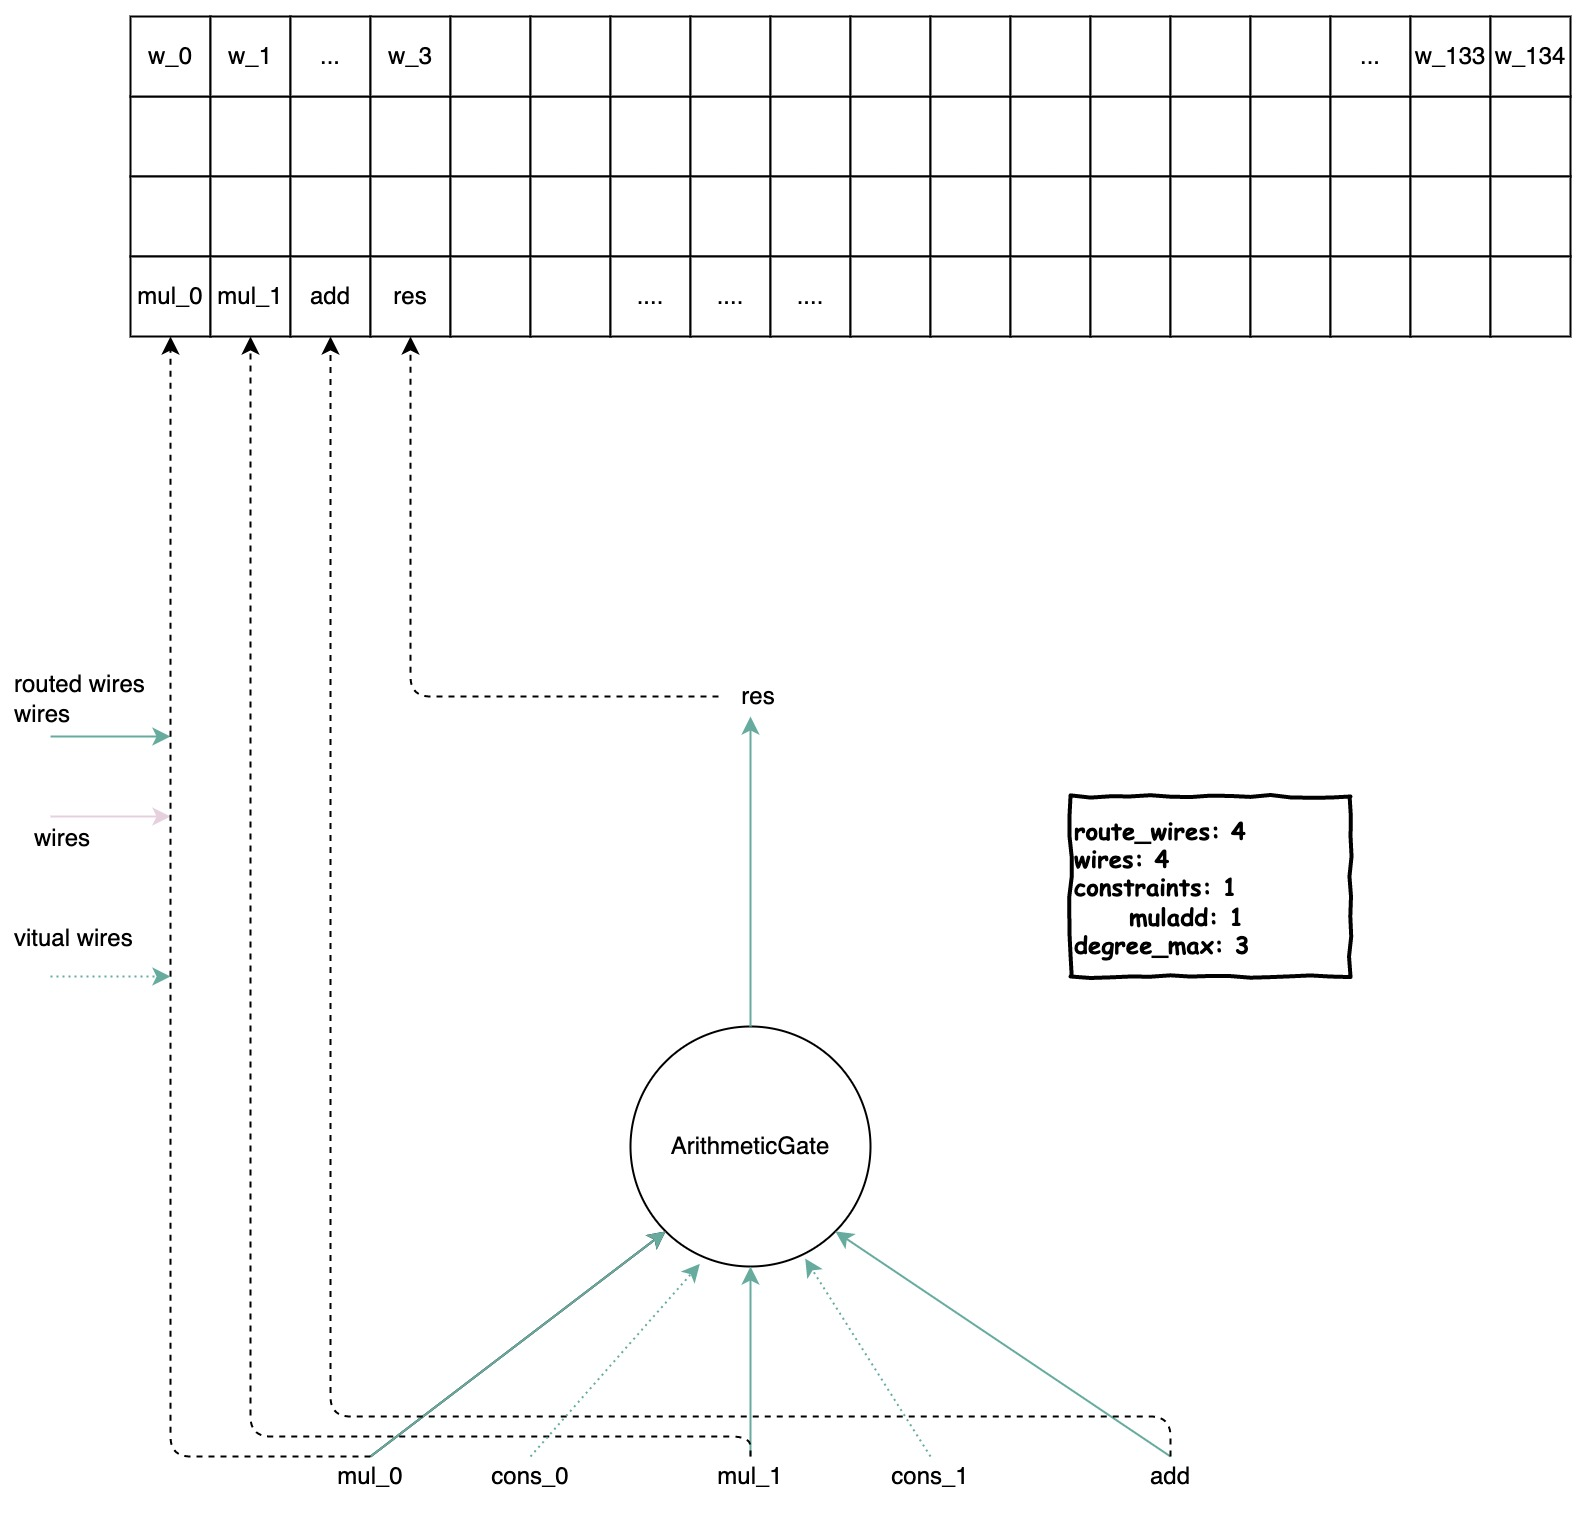
\includegraphics[width=0.8\textwidth]{gates/arithmetic_base.jpeg}
    \caption{ArithmeticGate}
    \label{fig:arthmetic-gate}
\end{figure}

There's only one constraint per operation, and degree is 3.